% !TEX encoding = UTF-8 Unicode
\documentclass[11pt,spanish]{article}\usepackage[]{graphicx}\usepackage[]{color}
% maxwidth is the original width if it is less than linewidth
% otherwise use linewidth (to make sure the graphics do not exceed the margin)
\makeatletter
\def\maxwidth{ %
  \ifdim\Gin@nat@width>\linewidth
    \linewidth
  \else
    \Gin@nat@width
  \fi
}
\makeatother

\definecolor{fgcolor}{rgb}{0.345, 0.345, 0.345}
\newcommand{\hlnum}[1]{\textcolor[rgb]{0.686,0.059,0.569}{#1}}%
\newcommand{\hlstr}[1]{\textcolor[rgb]{0.192,0.494,0.8}{#1}}%
\newcommand{\hlcom}[1]{\textcolor[rgb]{0.678,0.584,0.686}{\textit{#1}}}%
\newcommand{\hlopt}[1]{\textcolor[rgb]{0,0,0}{#1}}%
\newcommand{\hlstd}[1]{\textcolor[rgb]{0.345,0.345,0.345}{#1}}%
\newcommand{\hlkwa}[1]{\textcolor[rgb]{0.161,0.373,0.58}{\textbf{#1}}}%
\newcommand{\hlkwb}[1]{\textcolor[rgb]{0.69,0.353,0.396}{#1}}%
\newcommand{\hlkwc}[1]{\textcolor[rgb]{0.333,0.667,0.333}{#1}}%
\newcommand{\hlkwd}[1]{\textcolor[rgb]{0.737,0.353,0.396}{\textbf{#1}}}%
\let\hlipl\hlkwb

\usepackage{framed}
\makeatletter
\newenvironment{kframe}{%
 \def\at@end@of@kframe{}%
 \ifinner\ifhmode%
  \def\at@end@of@kframe{\end{minipage}}%
  \begin{minipage}{\columnwidth}%
 \fi\fi%
 \def\FrameCommand##1{\hskip\@totalleftmargin \hskip-\fboxsep
 \colorbox{shadecolor}{##1}\hskip-\fboxsep
     % There is no \\@totalrightmargin, so:
     \hskip-\linewidth \hskip-\@totalleftmargin \hskip\columnwidth}%
 \MakeFramed {\advance\hsize-\width
   \@totalleftmargin\z@ \linewidth\hsize
   \@setminipage}}%
 {\par\unskip\endMakeFramed%
 \at@end@of@kframe}
\makeatother

\definecolor{shadecolor}{rgb}{.97, .97, .97}
\definecolor{messagecolor}{rgb}{0, 0, 0}
\definecolor{warningcolor}{rgb}{1, 0, 1}
\definecolor{errorcolor}{rgb}{1, 0, 0}
\newenvironment{knitrout}{}{} % an empty environment to be redefined in TeX

\usepackage{alltt}
\usepackage[spanish,mexico]{babel}
\usepackage[utf8]{inputenc}
\usepackage{authblk}
\usepackage{setspace}
\usepackage[margin=1in]{geometry}
\usepackage{graphicx}
\usepackage{subcaption}
\usepackage{amsmath}
\usepackage[rightcaption]{sidecap}

\usepackage{natbib}
\bibliographystyle{apalike}

\usepackage{booktabs}
\usepackage[table,xcdraw]{xcolor}

\let\olditemize\itemize
\def\itemize{\olditemize\itemsep=0pt}

%%%%%% Title %%%%%%
% Full titles can be a maximum of 200 characters, including spaces. 
% Title Format: Use title case, capitalizing the first letter of each word, except for certain small words, such as articles and short prepositions
\title{\huge{Reporte de trabajo: Análisis de Redes con datos del Tamizaje para la detección de riesgos a la Salud Mental por Covid-19}}

%%%%%% Authors %%%%%%
\author[ ]{Elena Villalobos Nolasco}

%%%%%% Affiliations %%%%%%
%affil[ ]{}

%%%%%% Date %%%%%%
% Date is optional
\date{Enero, 2022.}

%%%%%% Spacing %%%%%%
% Use paragraph spacing of 1.5 or 2 (for double spacing, use command \doublespacing)
\onehalfspacing
\IfFileExists{upquote.sty}{\usepackage{upquote}}{}
\begin{document}

\maketitle

%%%%%% Main Text %%%%%%

El presente documento tiene los avances realizados en el proyecto de {\bf Análisis de Redes como alternativa de análisis para estudiar psicopatologías} y tiene como base principal el tutorial de \cite{main_tutorial}. En la primera parte del documento hablaremos de los conceptos básicos para entender el análisis de redes, así como de la descripción de los gráficos principales para estudiar las características de las redes. En la segunda parte presentaremos los resultados preliminares, con la base de datos del Tamizaje para la detección de riesgos. 


\section{Conceptos básicos para entender el análisis de redes}

El análisis de redes, basado en la teoría de grafos, es un método analítico que tiene como objetivo estudiar las interrelaciones existentes entre entidades. En éste, los nodos representan entidades (aeropuestos, personas, etc.), y las conexiones, también conocidas como aristas, son observadas, medidas y conocidas (número de vuelos entre aeropuestos, amistades, etc.). 

De manera similar pero estructuralmente diferente al análisis de redes, las redes psicológicas consisten en nodos que representan las variables observadas que están interconectados por aristas que representan relaciones estadísticas, las cuales se infieren a partir de los mismos datos. Por ejemplo, en un cuestionario psicométrico las respuestas a las preguntas son los nodos, y lo que se calcula son las interrelaciones, también entendidas como las aristas. Como dichas interrelaciones se estiman a partir de los datos, es muy recomendable tener más datos que ayuden a hacer cómputos más confiables.

A grandes rasgos, el análisis de redes psicológicas tiene dos pasos involucrados:

\begin{enumerate}
  \item Estimar el modelo estadístico sobre los datos, es decir, la estimación de la red con sus pesos correspondientes entre las variables observadas. 
  \item Analizar si las estimaciones de los pesos son adecuadas, a partir de medidas desarrolladas en teoría de grafos. 
\end{enumerate}


De manera específica, en las redes psicológicas {\bf los nodos representan las variables observadas y las aristas representan coeficientes de correlación parcial entre variables (i.e. pesos de las aristas), condicionadas sobre las otras variables observadas}. Para evaluar la importancia de los nodos en la red se computan las medidas de centralidad que son: 

\begin{description}
  \item[Fuerza del nodo:] que tan bien el nodo es {\bf directamente} conectado con otros nodos.
  \item[Closeness:] cuantificar que tan bien el nodo es indirectamente conectado a otros nodos. 
  \item[Betweeness:] que tan importante es un nodo en el camino promedio entre dos nodos. 
\end{description}

Dentro del tutorial de \cite{main_tutorial} ellos simularon una red con un modelo gráfico gausiano del cual obtuvieron las medidas de centralidad ya descritas, ambos presentados en la Figura \ref{fig:tuto_red}. En ésta se puede observar de lado derecho que las conexiones más fuertes positivas son entre los nodos 16 y 17, 3 y 4, y 11 y 5. También, se puede observar una conexión negativa entre los nodos 10 y 12. En cuanto a las medidas de centralidad, el nodo 17 y el 3 salen como los más importantes para la red, tanto para la fuerza del nodo como para \emph{betweenness}. 

\begin{figure}[!ht]
\centering
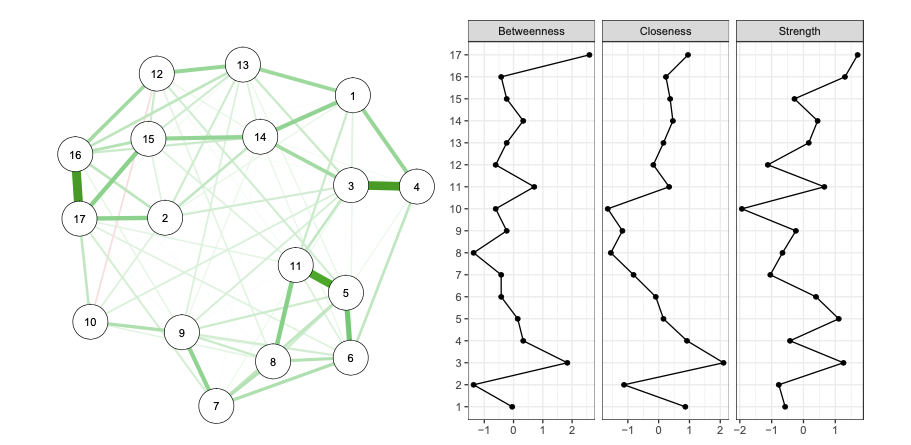
\includegraphics[scale=0.5]{images/red_medidas_tutorial}
\caption{Red de modelo gráfico gausiano del cuestionario PTSD con 17 reactivos (panel derecho) y sus respectivos índices de centralidad (panel derecho), presentados en el tutorial de \cite{main_tutorial}}
\label{fig:tuto_red}
\end{figure}

A partir de los parámetros obtenidos del modelo anterior se simularon datos de 500 sujetos más. Se observó que la red que se generó era muy similar a la original. Sin embargo, se encontró que las medidas de centralidad difieren mucho entre las simulaciones y el modelo original. Por lo que destacaron la importancia de evaluar la precisión de las estructuras de las redes psicológicas, y para ello sugieren los siguientes tres pasos: 

\begin{enumerate}
  \item Estimar la precisión de los pesos de las aristas, utilizando Intervalos de Confianza con bootstrap.
  \item Evaluar la estabilidad de los índices de centralidad observados sobre sub-conjuntos de datos.
  \item Realizar tests de diferencias significativas entre los pesos de las aristas y los índices de centralidad. 
\end{enumerate}

Antes de presentar la evaluación de la precisión de las redes, en la siguiente sección destacaremos algunas partes importantes sobre el análisis de redes.

\subsection*{Especificaciones de estimaciones de redes psicológicas.}

Un modelo de redes que se usa popularmente para estimar redes psicológicas es un Campo Aleatorio de Markov por Pares (Pairwise Markov Random Field, PMRF). En este modelo, los nodos representan variables, y se conectan a través de arístas no-direccionadas, indicando dependencia condicional entre dos variables; si dos varialbes que no están conectadas son independientes, aún después de condicionar sobre las otras variables. Cuando los datos son normales multivariados, esta independencia condicional correspondería a una correlación parcial igual a cero. 

Cuando los datos son binarios, el modelo PRMF a utilizar es el modelo Ising. Mientras que si los datos siguen una densidad normal multivariada, el modelo apropiado de PRMF, es el modelo gráfico gausiano (GGM), en los que las aritas pueden ser directamente interpretadas como coeficientes de correlación parcial. El GGM requiere un estimado de la matriz de covarianza como entrada, que en caso de que los datos sean ordinales se pueden utilizar correlaciones policóricas (i.e. correlación para variables ordinales de variables latentes).

El modelo PMRF tiene el problema de que el número de parámetros a estimar crece mucho con el tamaño de la red y en generalmente en el área de psicología no se tienen tantos datos que compensen esta sobre-estimación. Para tratar dicho problema se utiliza la forma de regularización de LASSO (Least Absolute Shrinkage and Selection Operator), técnica penaliza el uso de muchos parámetros, limitando la suma de valores paramétricos absolutos. Por lo que LASSO regresa un modelo de red más conservador, que en otras palabras, sólo un pequeño número de aristas se utilizan para explicar la covariación de la estructura en los datos\footnote{El paquete de \texttt{qgraph} utiliza lasso en combinación con la selección de modelos EBIC para estimar un GGM regularizado.}. 


\subsection{Precisión de los pesos de las aristas}

Para evaluar la variabilidad de los pesos de las aritas se pueden estimar Intervalos de Confianza\footnote{Para construir Intervalos de Confianza se necesita saber la \emph{distribución muestral} del estadístico de interés. Sin embargo, saber dicha distribución para medidas de centralidad, es difícil por su misma complejidad de cómputo. Por lo que se utiliza bootstrap, que es una técnica que implica estimar repetidamente un modelo con datos muestreados o simulados para obtener el estadístico de interés. Se puede hacer bootstrap de dos maneras, paramétrico y no parámetrico. En el \emph{no paramétrico}, las observaciones de los datos se re-muestrean con reemplazo para crear un nuevo conjunto de datos, mientras que el \emph{paramétrico} muestrea nuevas observaciones del modelo paramétrico que fue estimado a partir de los datos originales, lo que crea una serie de valores que pueden ser utilizados para estimar la distribución muestral.} con la técnica de re-muestreo bootstrap. Se aconseja que para datos ordinales, se utilice bootstrap no paramétrico. 

Es importante mencionar que los resultados del bootstrap no deberían ser utilizados para hacer test de significancia diferente de cero, pues la regularización de LASSO ayuda a quitar los pesos que no son importantes en la red. Esto significa que los pesos que aparecen dentro de la red, ya pueden ser significativamente diferentes de cero, por lo que conviene considerarlos como importantes. 

Entonces la interpretación de los Intervalos de Confianza con bootstrap para los pesos de las aristas no se deben asumir diferentes de cero, si no que este sólo muestra la precisión de esos pesos y lo que se debe de hacer es comparar los valores de las aristas entre ellos. Cuando un intervalo es ancho, es difícil hacer la interpretación de la fuerza del nodo, por lo que probablemente resultará en poca precisión para las otras medidas de centralidad. 

La Figura \ref{fig:inter_boot_tutorial} son los Intervalos de Confianza para el modelo presentado al inicio de este documento (figura \ref{fig:tuto_red}). En este gráfico cada línea horizontal representa una arista de la red, ordenadas desde la arista con el peso más alto, hasta la arista con el peso más bajo. Es decir, las conexiones colocadas en la parte superior del gráfico son las más fuertes, que son entre los nodos 17 y 16, 3 y 4, y 11 y 5. Se podría considerar que son, de manera confiable, las tres aristas con más fuerza de conexión debido a que sus Intervalos de Confianza no se superponen con los CI de ningún otro borde.

\begin{figure}[!ht]
\centering
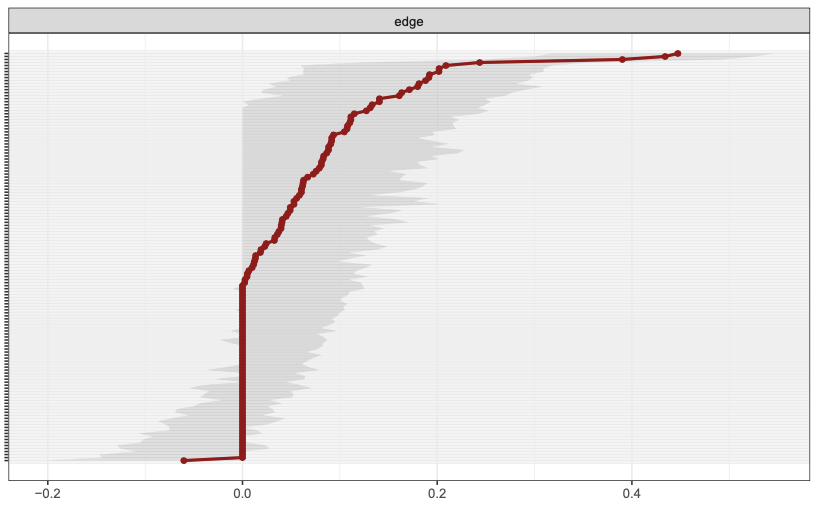
\includegraphics[scale=0.5]{images/intervalos_boot_tutorial}
\caption{Intervalos de Confianza bootstrap de \cite{main_tutorial}}
\label{fig:inter_boot_tutorial}
\end{figure}

\subsection{Estabilidad de centralidad}

Para saber la estabilidad de las medidas de centralidad no se puede utilizar bootstrap\footnote{Esto es porque se generan distribuciones muestrales sesgadas.}, por lo que se propone estudiar dichas medidas con subconjuntos de datos. Se dice que los índices de centralidad son estables cuando el orden de los índices es el mismo en diferentes submuestras del mismo conjunto de datos. Lo que se hace es que se aplica la técnica de re-muestreo (el bootstrap regular) para diversas proporciones de los mismos participantes (o variables) y se evalúa si la correlación entre los índices de centralidad originales y aquellos obtenidos en las submuestras son estables. Si la correlación cambia completamente después de quitar 10\% de la muestra, por ejemplo, entonces las interpretaciones de centralidad pueden ser erróneas. A esto se le llama bootstrap de subconjuntos con \emph{case-dropping}. Para cuantificar dicha estabilidad se propone la medida de coeficiente de estabilidad de correlación (CS-coefficient), que se recomienda sea mayor a 0.7.


La Figura \ref{fig:estabilidad_tutorial}, muestra la estabilidad de las medidas de centralidad del modelo que se ha venido presentando. Este, como se menciona, debe de permanecer estable y tener promedio de correlación similar entre los diferentes porcentajes de muestra. Por lo tanto, se espera que las líneas se mantengan rectas y en la parte superior, a lo largo de los porcentajes, que están en el eje x. Para este caso, la medida de fuerza parece ser la más estable, mientras que \emph{betweennes} y \emph{closeness}, tienen mayor disminución en cuanto se reduce el porcentaje que muestra. 

\begin{figure}[!ht]
\centering
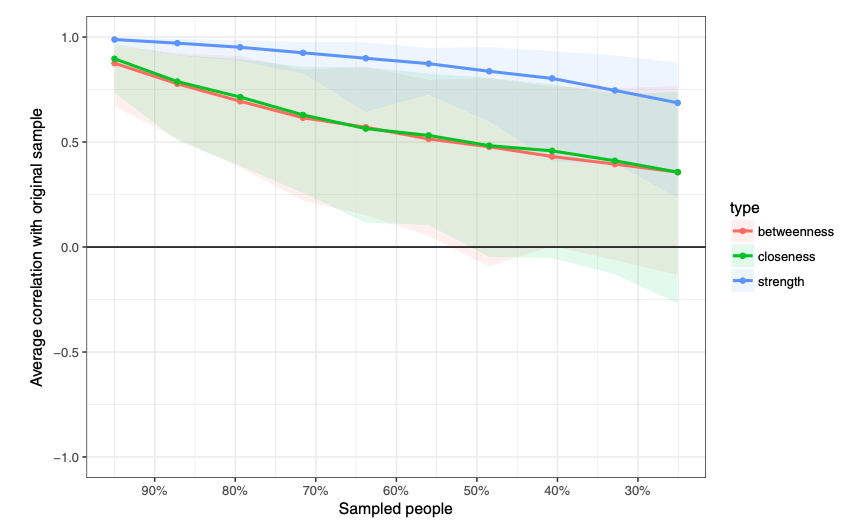
\includegraphics[scale=0.5]{images/estabilidad_tutorial}
\caption{Estabilidad de las mendidas de centralidad del ejemplo del tutorial.}
\label{fig:estabilidad_tutorial}
\end{figure}

\subsection{Test para diferencias significativas}

El test de diferencias significativas, que también se hace con bootstrap, se utiliza para saber si una arista es significativamente distinta de otra, o si las medidas de centralidad son significativamente distintas de otras. En este test se recomienda, tener cuidado en la interpretación debido a que el no rechazar la hipótesis nula, no es evidencia de que la hipótesis alternativa sea verdadera\footnote{Hipótesis nula: no hay diferencias.}.


\section{Resultados preliminares}

Los siguientes gráficos se presentan a partir de la red




 



\newpage


\bibliography{bibtex}

\end{document}
